\begin{appendices}

    \chapter[Jira : L'outil pour la gestion de projet]{Jira : L'outil essentiel pour la gestion quotidienne de projet}\label{ch:jira}

    \begin{figure}[h]
        \centering
        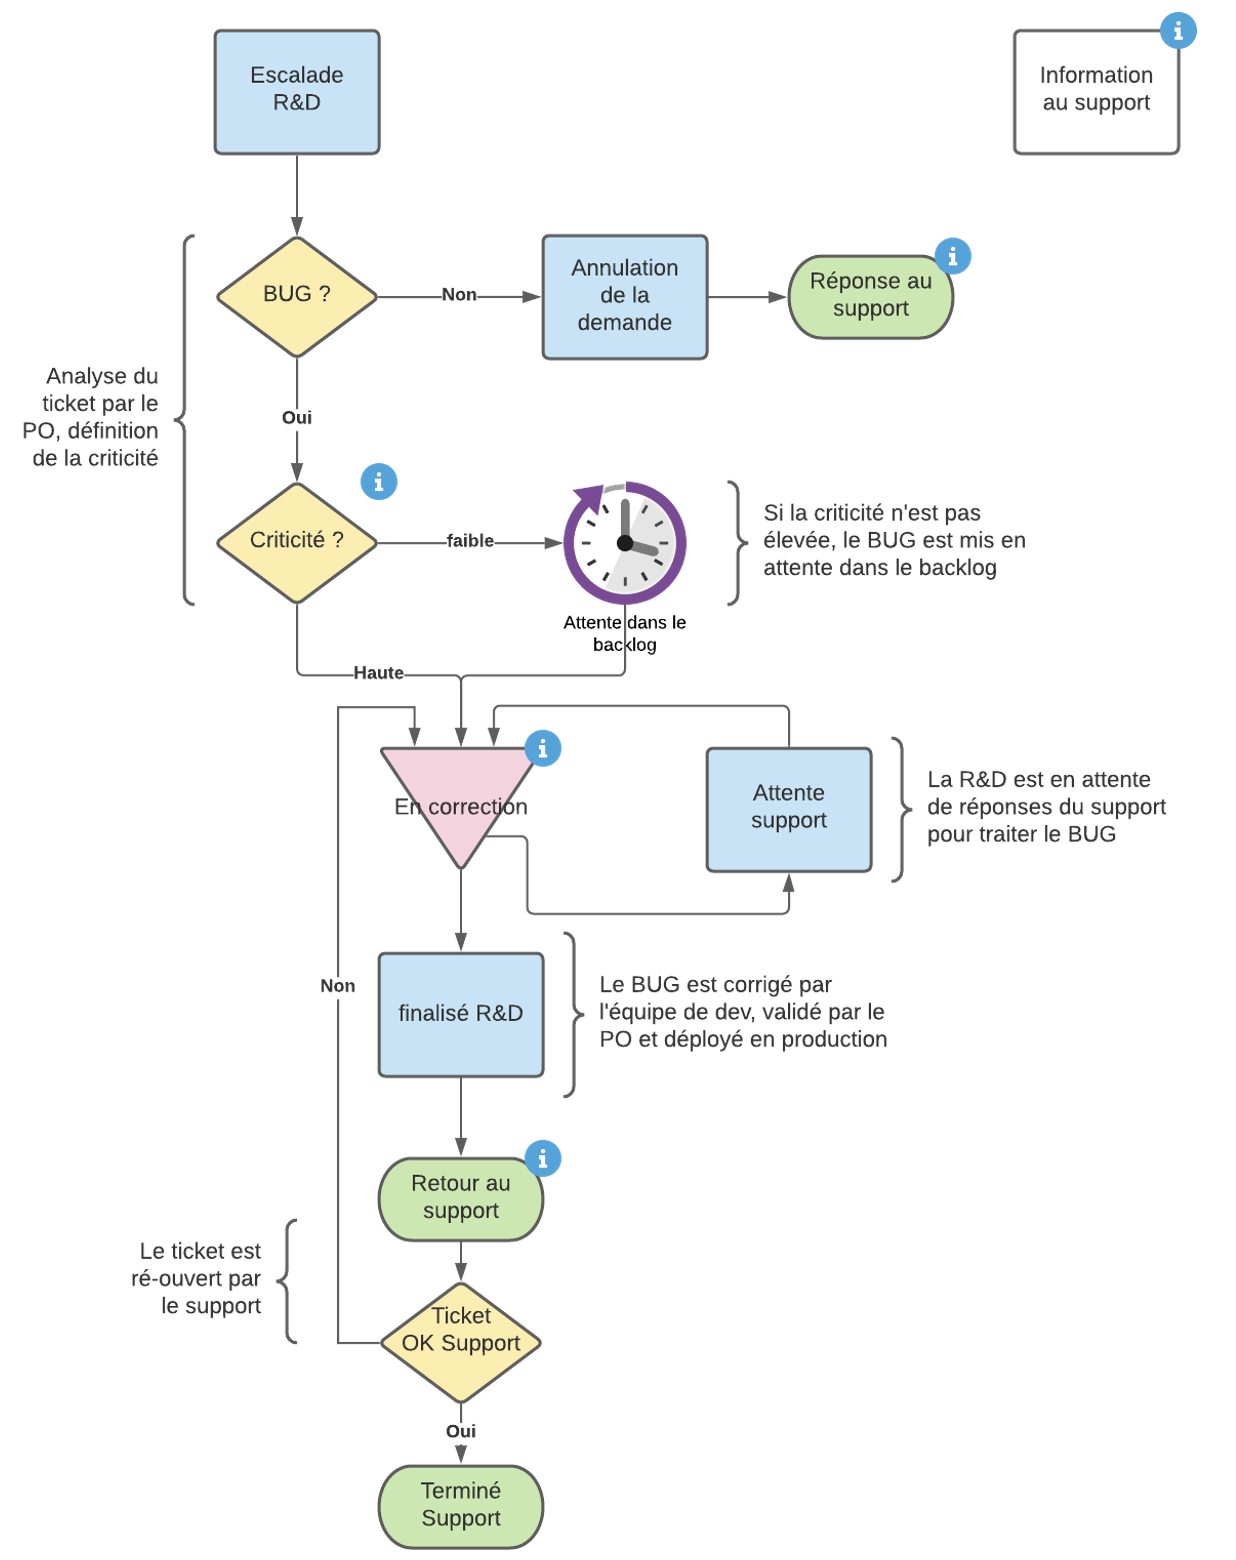
\includegraphics[width=0.91\textwidth]{img/lifecycle-of-bugs}
        \caption{Diagramme d'activité du traitement des bogues.}
        \label{fig:lifecycle-of-bugs}
    \end{figure}

    \begin{figure}[h]
        \centering
        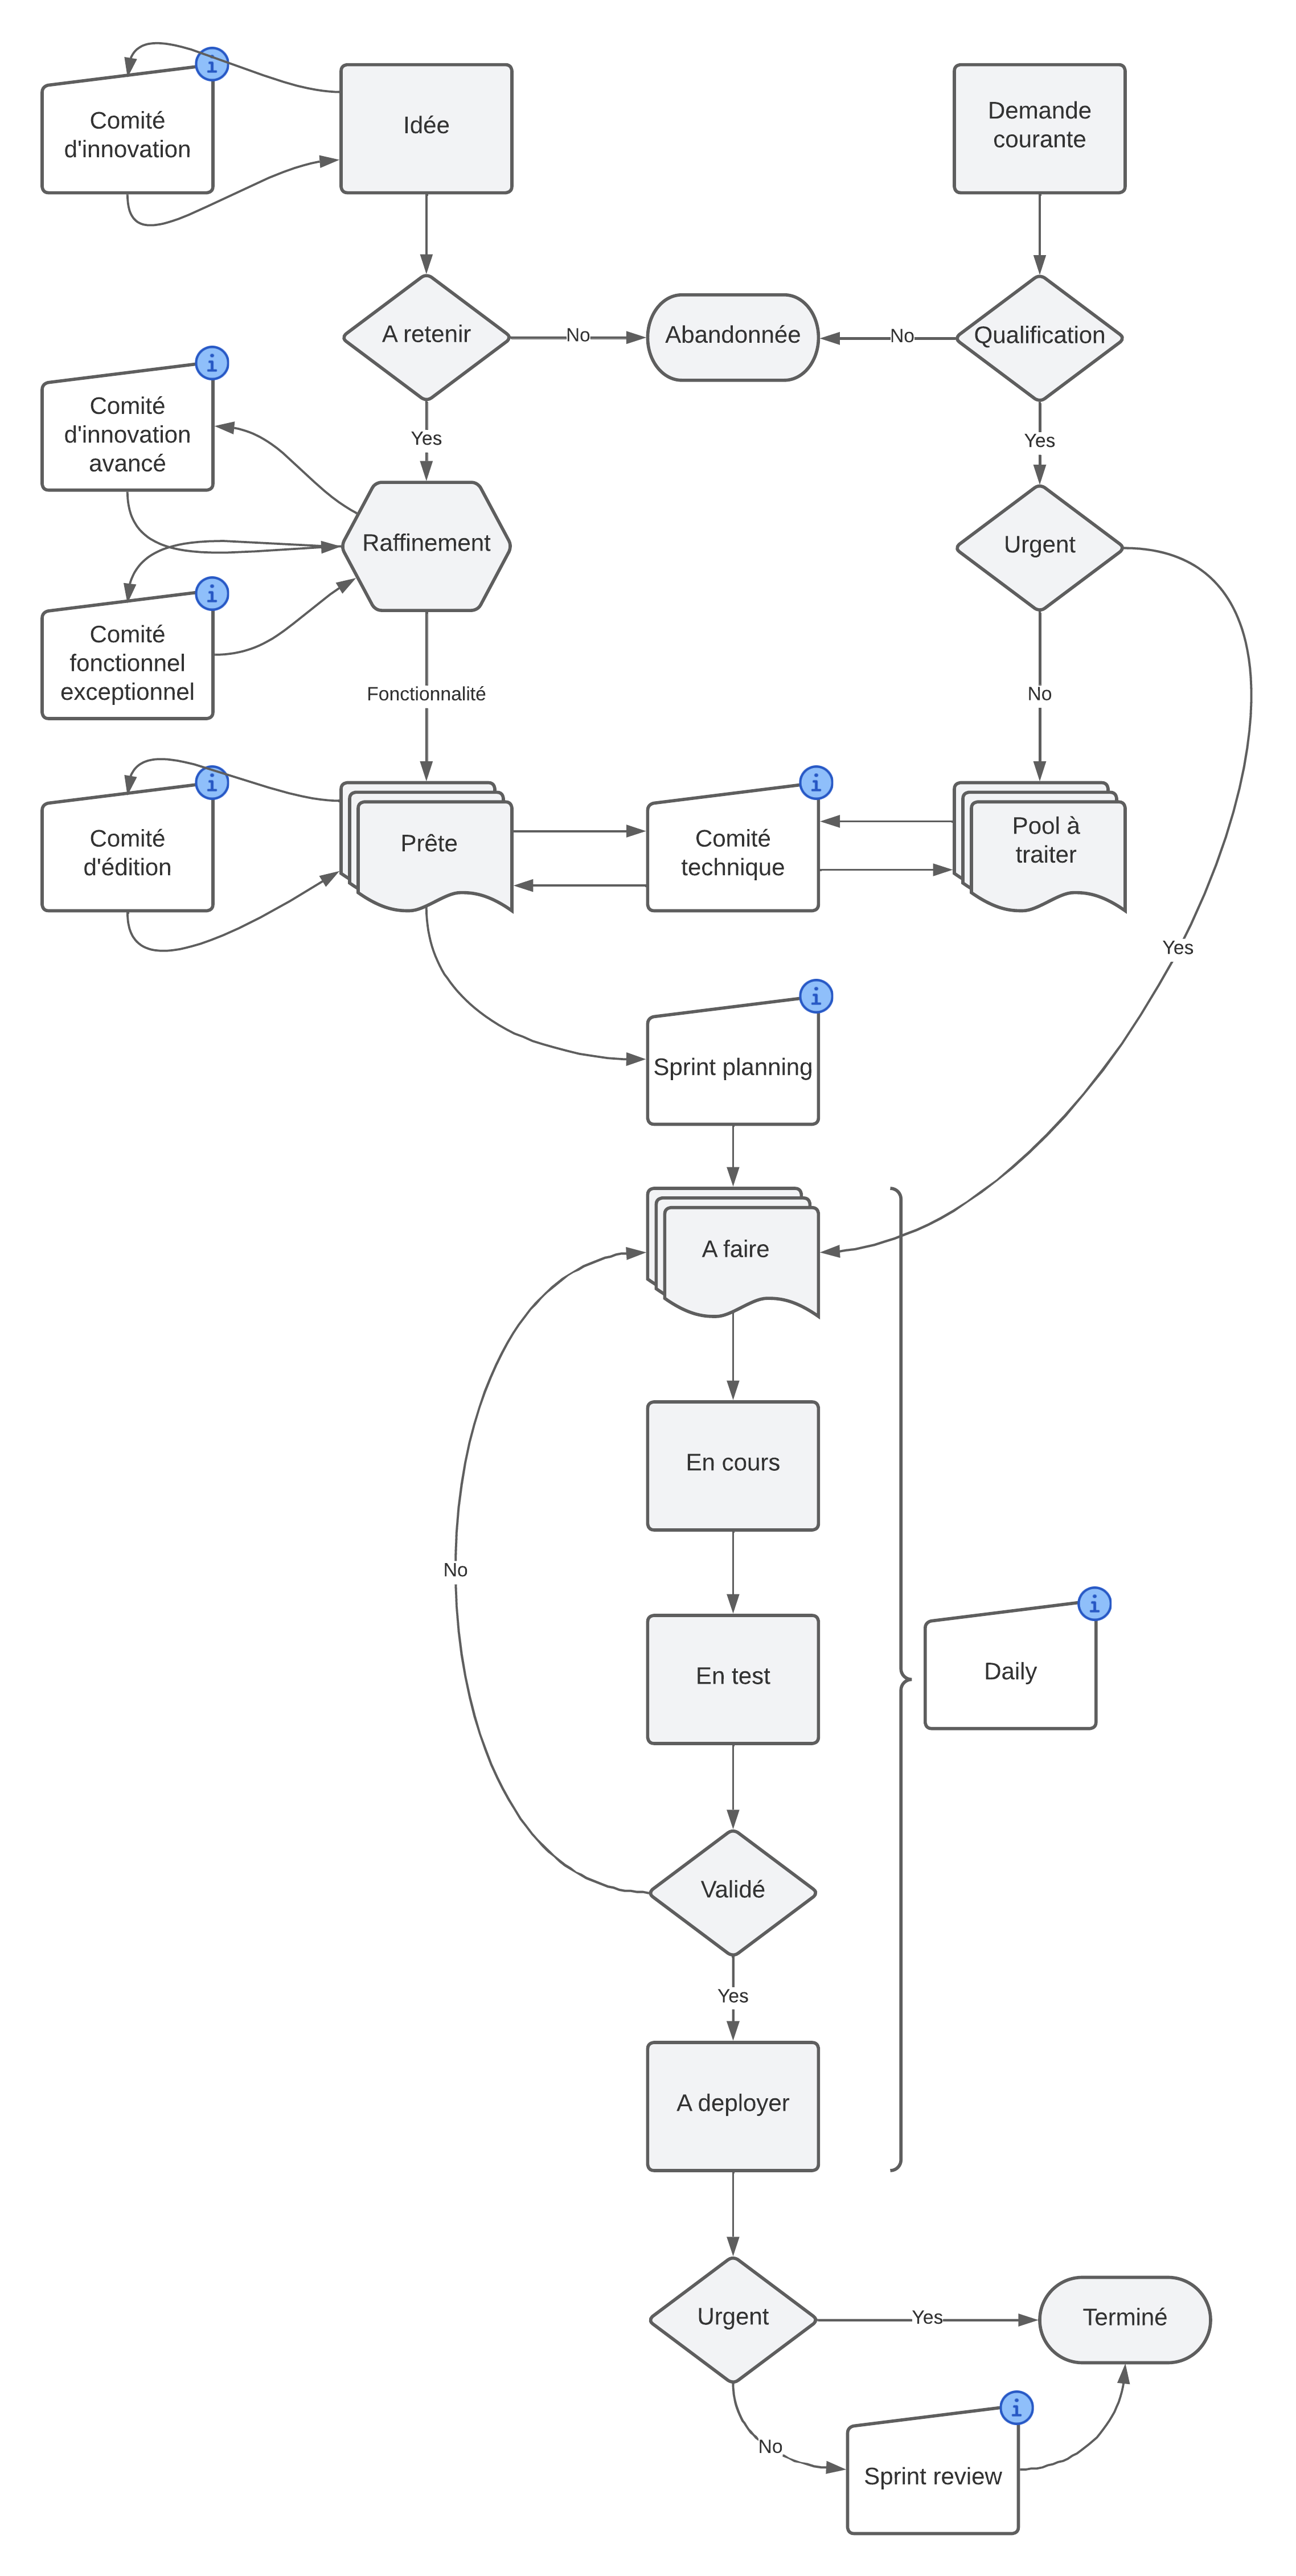
\includegraphics[height=0.94\textheight]{img/lifecycle-of-incoming-ideas}
        \caption{Diagramme d'activité du traitement des idées et des bogues (demandes courantes) entrants chez SuiviDeFlotte.}
        \label{fig:lifecycle-of-incoming-ideas}
    \end{figure}

    \begin{figure}[h]
        \centering
        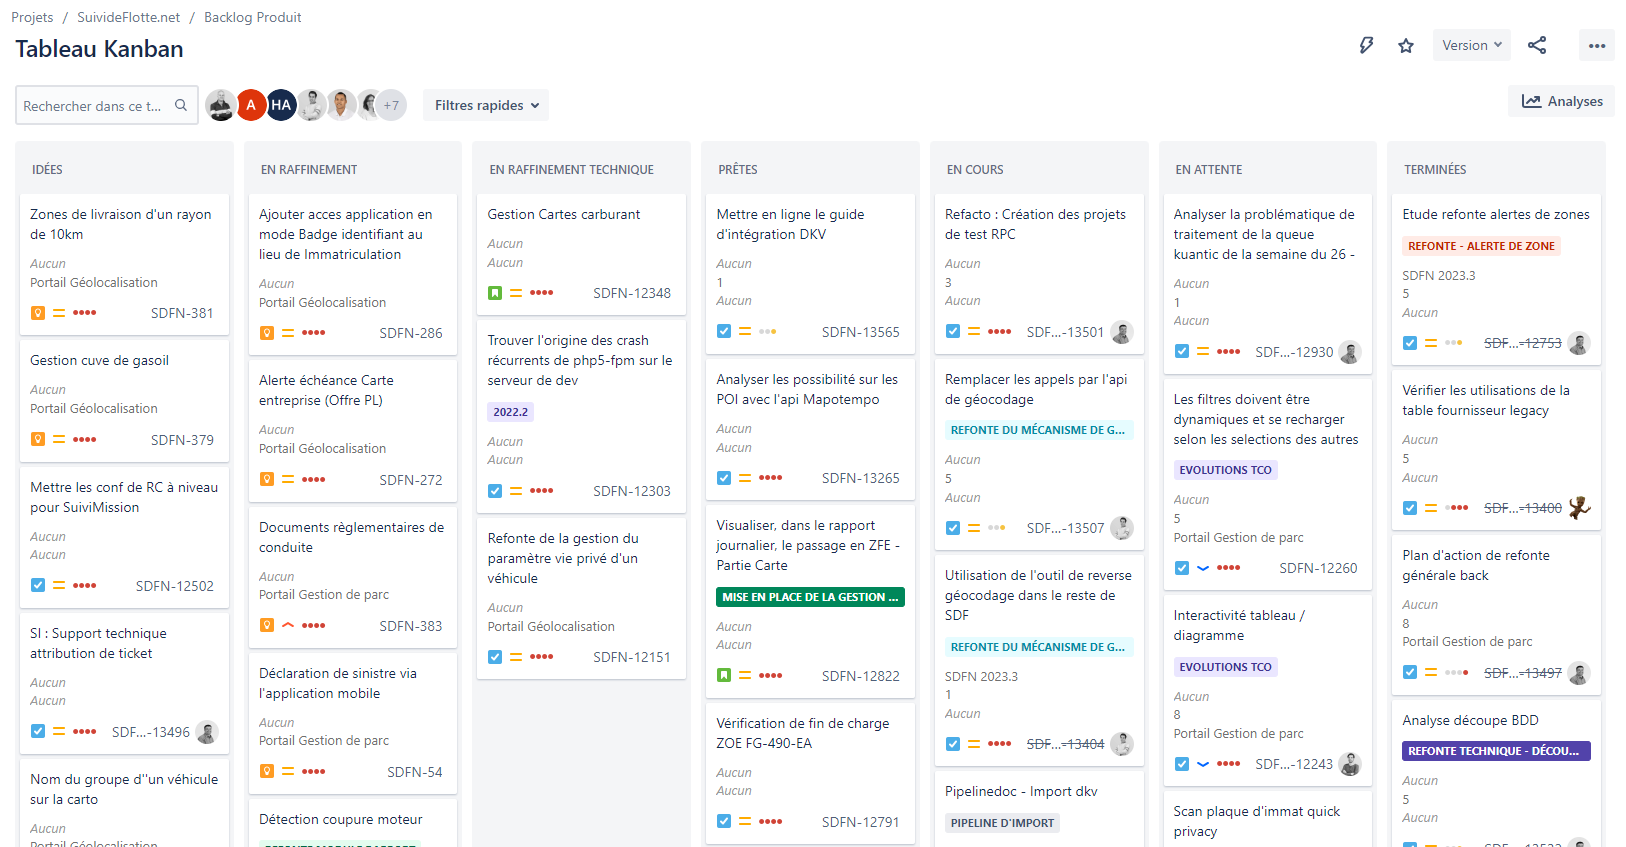
\includegraphics[width=\textwidth]{img/product-backlog}
        \caption{Le Backlog de produit sous forme de tableau Kanban dans Jira.}
        \label{fig:product-backlog}
    \end{figure}

    \begin{figure}[h]
        \centering
        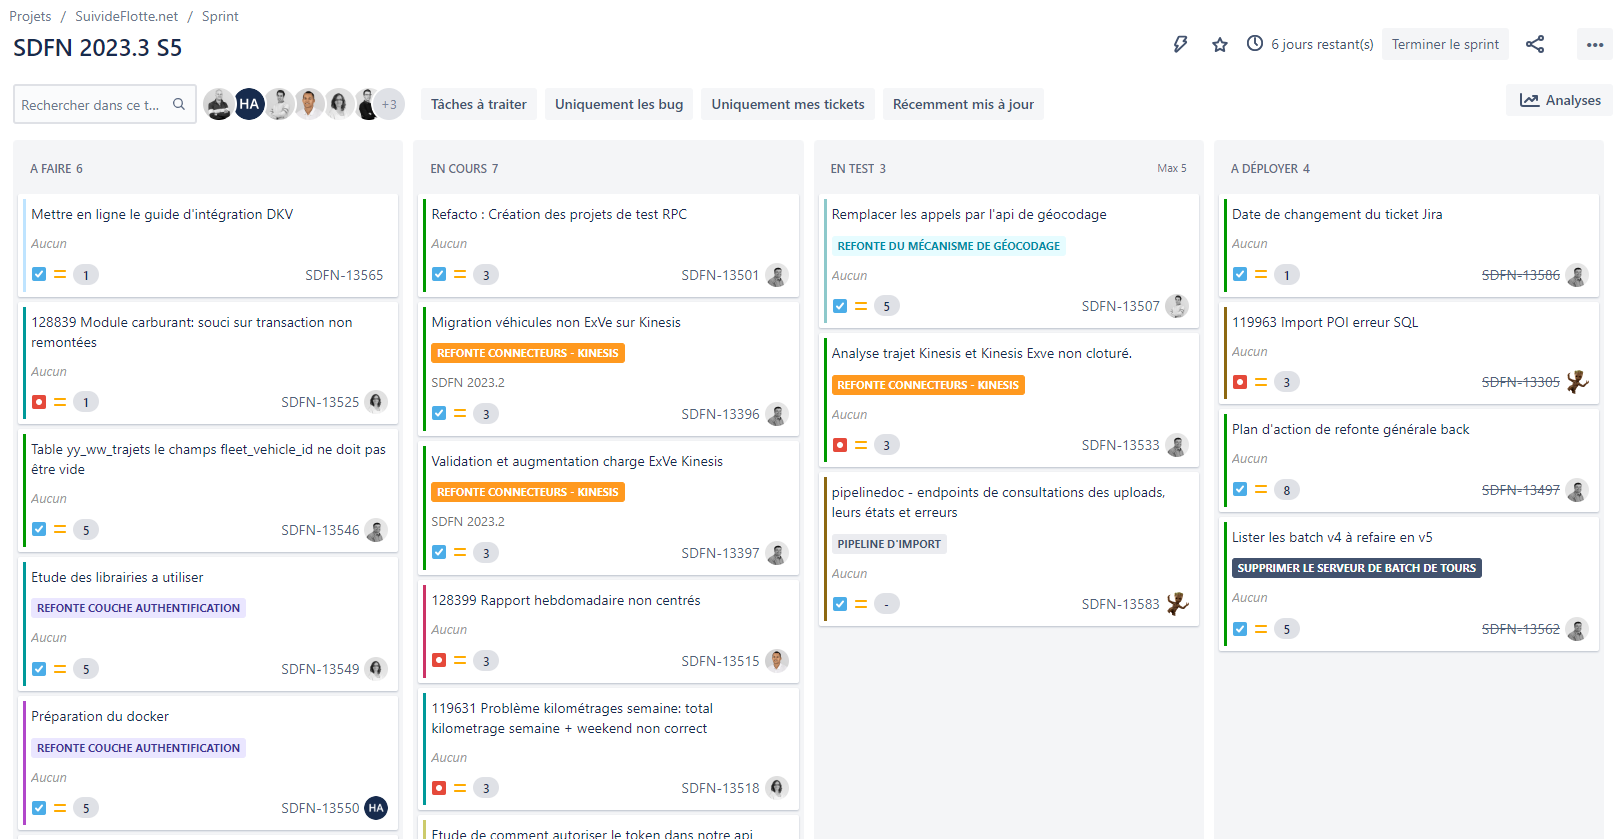
\includegraphics[width=\textwidth]{img/sprint}
        \caption{Le Backlog de sprint sous forme de tableau Kanban dans Jira.}
        \label{fig:sprint}
    \end{figure}

    \begin{figure}[h]
        \centering
        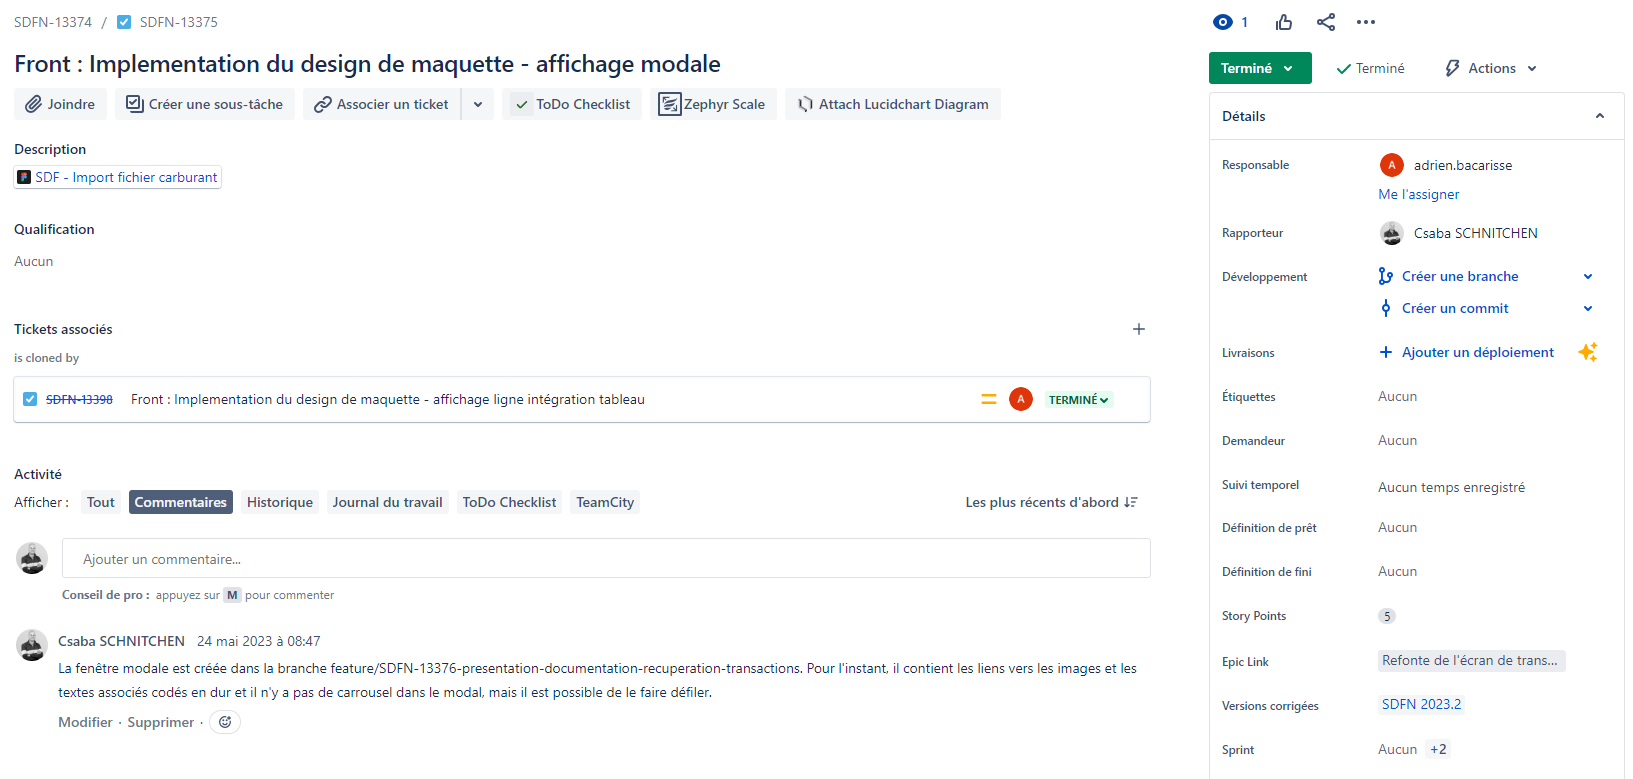
\includegraphics[width=\textwidth]{img/ticket}
        \caption{Un exemple de ticket dans Jira pour le projet d'amélioration de la page d'importation des fichiers des transactions de carburant.}
        \label{fig:ticket}
    \end{figure}

\end{appendices}